\documentclass[letterpaper, 12 pt, conference]{IEEEtran}  
\IEEEoverridecommandlockouts                              
%\overrideIEEEmargins
\usepackage[utf8]{inputenc}
\usepackage[T1]{fontenc}
\usepackage{hyperref}
\usepackage{xcolor}
\usepackage{graphicx}
\usepackage{amsmath}
\graphicspath{{./images/}} 


\begin{document}
\title{Expectation Maximization $|$ Hidden Markov Model $|$ EM framework}
% author names and affiliations
\author{\IEEEauthorblockN{Vaishnav Mukesh}
\IEEEauthorblockA{202051196}
\and
\IEEEauthorblockN{Kaushik Rathva}
\IEEEauthorblockA{202051156}
\and
\IEEEauthorblockN{Patel Jaykumar}
\IEEEauthorblockA{202051136}
\and
\IEEEauthorblockN{Sontakke Ajinkya}
\IEEEauthorblockA{202051179}
}

\maketitle
%\thispagestyle{empty}
%\pagestyle{empty}

\setlength{\parindent}{20pt}
\noindent Github link: \href{https://github.com/JARVIS-codebase/LAB-6}{LAB-6} \\ \\
\indent \begin{abstract}
Implementing the Expectation Maximization routine for learning parameters of a Hidden Markov Model is required in order to use the EM framework to build algorithms for issues with hidden or incomplete information.
\end{abstract}

\section{Introduction}
A Markov model is a technique for modifying systems that have the Markov attribute randomly.
As a result, the next state is simply dependent on the current state and is independent of everything that occurred in the past at any particular time.\\
\section{Hidden Markov Model}
\indent The HMM is used to simulate systems where the system's state varies over time and can only be inferred from the output. Given a series of observations, the purpose of HMM is to estimate the underlying state sequence. Algorithms like the Viterbi Algorithm, the Forward-Backward Algorithm, or the Baum-Welch Algorithm are frequently used for this.\\
\section{Solution}
\indent From the reference "A Revealing Introduction to Hidden Markov Models", we calculated $\alpha$-pass, $\beta$-pass, di-gammas for re-estimating the state transition probability matrix (A), observation probability matrix (B), initial state distribution ($\pi$) for Leo Tolstoy’s book War and Peace. We re-estimated A,B and ($\pi$) based on the observed sequence O, taking initial values for A, B and $\pi$ and calculating $\alpha$, $\beta$, the di-gammas and log probability for the data i.e. War and Peace. We took letters from the book after removing all the punctuation and converting the letters to lower case. We initialized each element of $\pi$ and A randomly to approximately 1/2. The initial values are:\\
\[A:\begin{bmatrix}
0.47468 & 0.52532\\
0.51656 & 0.48344
\end{bmatrix}\] \\
Each element of B was initialized to approximately 1/27.\\
\[\pi:\begin{bmatrix}
0.51316 & 0.48684
\end{bmatrix}\]
After initial iteration,\\
\[log([P(O|\lambda)]) = -142533.41283009356\]\\ \\
After 100 iterations,\\
\[log([P(O|\lambda)]) = -138404.497179602\]\\
\subsection{Problem 2}
\noindent Expectation Maximization Algorithm:\\
With measurement data U, Expectation Maximization is an iterative optimization technique used to estimate some latent parameters.\\
\indent The Expectation Maximization Algorithm will be used to compute the biases of the 10 biased coins in the challenge.\\ \\
Expectation step:\\
We begin by speculating on the initial biases of the coins. The coin that was most likely to produce each set of outputs is then revealed. The Expectation Step is this.\\
Maximization step:\\
The new thetas are then calculated under the assumption that these values are accurate.This is referred as the Maximization Step.\\
Once the values converge, we simply repeat the Expectation and Maximization processes.

\subsection{Problem 3}
In this instance as well, we begin with an educated approximation for the two clusters and iterate to raise the values until convergence.\\
Expectation step:\\
We determine the likelihood that each point belongs to a specific cluster for each one.\\
Maximization step:\\
Based on the probabilities determined in the Expectation stage, we update the model parameters.\\
Once the values converge, we simply repeat the Expectation and Maximization processes. Likewise, give points to the cluster that has the highest likelihood.\\

\section{Observations}
\begin{enumerate}
    \item First Problem: 
     In the first problem after 100 iterations all the alphabets are divided into two states/groups i.e. vowels and consonants.\\ \\
    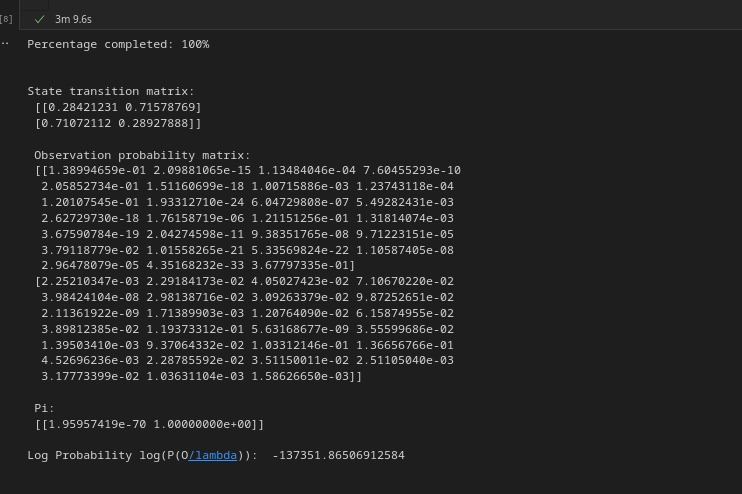
\includegraphics[scale=0.3]{images/6.1.jpg}\\ \\
    From above fig., we can clearly see that vowels are in first group and consonants are in second group. \\
    \item Second Problem: 
    We can see the initialized values of biases for all coins in Fig 2.\\
    And the final converged values of iterations of biases can be seen in Fig 3.\\
    The last row in Fig. 3. are our final values of biases for the coin.\\ \\
    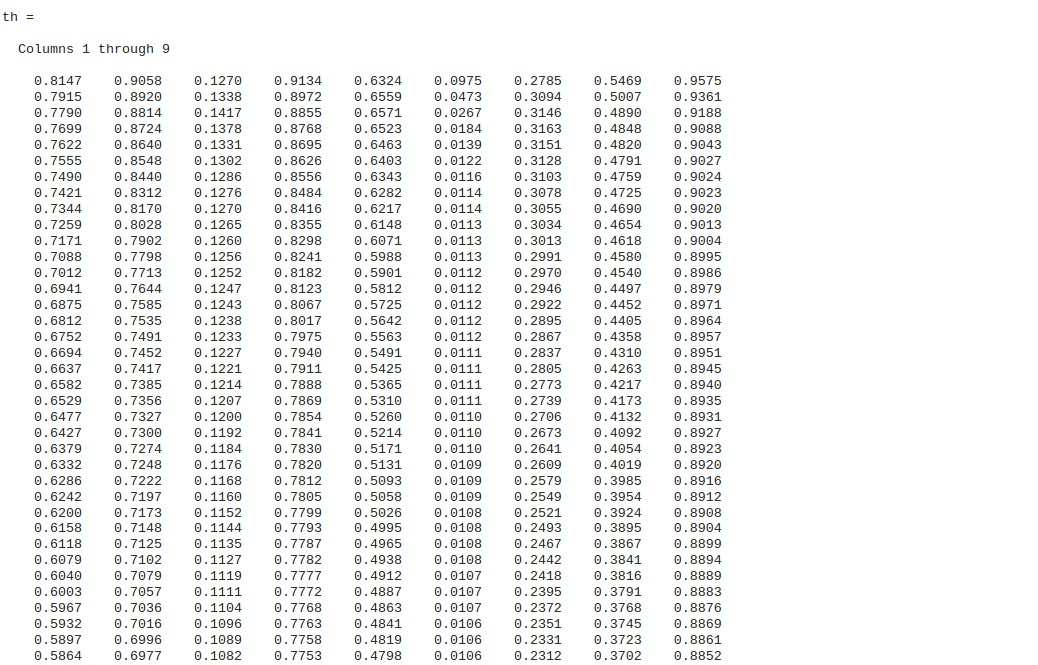
\includegraphics[scale=0.3]{images/6.2.jpg} \\ \\
    \item Third Problem: 
   Following the iterations, we discovered that two clusters had formed. Which point corresponds to which cluster might be foreseen.\\
    \indent Because we guess the initial values in K-means, it is an EM algorithm. It is possible to think of assigning data to the closest cluster centre as an E step and changing the centre values as a M step.\\ K-means is an EM method that assigns points to clusters based on latent factors.
\end{enumerate}
\begin{thebibliography}{}
\bibitem{}
Mark Stamp (2018) \emph{A revealing introduction to hidden markov models.}
\bibitem{}
Chuong B Do and Serafim Batzoglou (2008) \emph{What is the expectation maximization algorithm?}, Nature Biotechnology, Vol 26, Num 8, August 2008
\bibitem{}
Tanmay Ambadkar (2021) Artificial Intelligence Course. \\
\href{https://github.com/TanmayAmbadkar/CS302-AI/tree/master/Lab6}{https://github.com/TanmayAmbadkar/CS302-AI/tree/master/Lab6}(2023).
\end{thebibliography}
\end{document}